\documentclass[tikz,border=4pt]{standalone}
\usepackage{fontspec}
\setsansfont{texgyreheros-regular.otf}
\definecolor{room}{HTML}{234D50}\definecolor{line}{HTML}{889C96}
\begin{document}
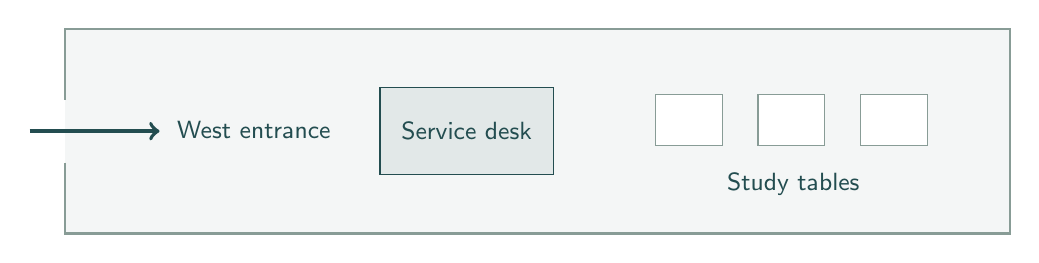
\begin{tikzpicture}[font=\sffamily\small,x=1cm,y=1cm]
  \fill[room!5] (0,0) rectangle (12,2.6);
  \draw[line,line width=.8pt] (0,.9)--(0,0)--(12,0)--(12,2.6)--(0,2.6)--(0,1.7);
  \draw[room,line width=1.4pt,->] (-.45,1.3)--(1.2,1.3);
  \node[anchor=west,text=room] at (1.3,1.32) {West entrance};
  \draw[room,fill=room!13] (4.0,.75) rectangle (6.2,1.85);
  \node[text=room] at (5.1,1.3) {Service desk};
  \foreach \x in {7.5,8.8,10.1}{
    \draw[line,fill=white] (\x,1.12) rectangle ++(.85,.65);}
  \node[text=room] at (9.25,.62) {Study tables};
\end{tikzpicture}
\end{document}
